\chapter{Design Details for Evolution Scenarios}
%TODO "describes the adaptive evolution scenari of.." changed to "changes in "
In this chapter we provide the detailed design documentation for each of the evolution scenarios
introduced in the prior section. Sec. \ref{App} sketches the design decision for the Mobile App that provides a second sales channel next to the existing Pick-up Shop. Sec. \ref{Docker} describes the adaptive cahnges of setting up a Docker environment to simplify the update process. They are both based on, or at least use the Hybrid Cloud-based Variant of CoCoME \cite{SWB-469002735}. In contrast, Sec. \ref{MS} provides a detailed design documentation of a new architectural version of CoCoME. This perfective evolution scenario is realized based on the Microservice idea.

\section{Design Decisions for the Mobile App} \label{App}
	%TODO Add most important information od App-Paper


\section{Setting up a Docker environment} \label{Docker}
	%TODO Add most important information of docker paper
	Looking to the changes for the Docker project, you can see in figure \ref*{techStack} the changes are affecting the technology stack in the form of adding additional layers. More detailed, the given CoCoME project is moved into the Docker Deamon, which runs a Linux distribution.The original parts of the stack, like Glassfish and the Java Virtual Machine, are still a part of the stack.\\
	\begin{figure}[H]
		\centering
		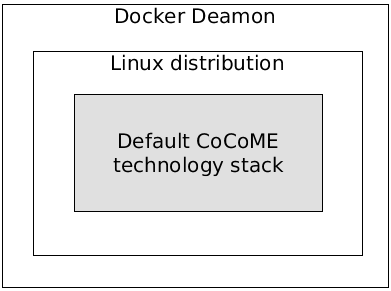
\includegraphics[width = 0.5\textwidth]{img/tech_stack_CoCoME.png}
		\caption{Extended technology stack CoCoME}
		\label{techStack}
	\end{figure}
	
	%TODO important here?
	The Dockerfile defines an environment based on the latest version of Ubuntu 16:04. Onto it there is installed Maven, Git and Java by using the Ubuntu package manager.\\
	Git has two purposes: On the one hand it is used to download the most recent version of CoCoME.	On the other hand, it is used to download a prefabricated version of Glassfish that already includes domains and other adjustments required for CoCoME. Java is required by Glassfish and CoCoME as they need the Java Virtual Machine. Maven is needed to deploy the latest version of CoCoME onto the provided Glassfish servers.
	
	
	During the development, it was decided to implement and provide two different versions. The first version always pulls the most recent CoCoME source code from GitHub, downloads the entire dependencies with maven, compiles and builds the project and finally, deploys CoCoME on the Glassfish servers. . As a consequence. creating and starting a Docker Container takes about one hour.\\
	In contrast, the second version only  pulls a prefabricated version of CoCoME from GitHub. Therefore, pulling the source code up to building the project is skipped. As a consequence, Maven does not have to be included in the technology stack. Solely, deploying CoCoME on the glassfish server is necessary.\\
	This reduces the deployment time to a few minutes but has a disadvantage: The prefabricated version is updated manually. Therefore, it is sometime not the most recent version.\\
	By providing both, a fast deploying version and a current version, the user can choose whats the best for its situation.
	

	

	
\section{Using Microservices Technology} \label{MS}
	\begin{itemize}
		\item je microservice absatz mit entsprechenden Sequenzendiagram %fertig machen der implementierung
		\item frontend? muss dazu auch das gemacht werden?
		\item ein blocktext zu mehereren diagrammen oder diagramme zwischen text?
		
	
			\item je die einzelnen module und szenarien erlaeutern in dem diese sinnvoll sind
	\end{itemize}
	
		\subsubsection{Products}
		abstrahieren der Produktinformationen 
		
		\subsubsection{Stores}
		einzelne Laeden alleinstehend abbilden um nach bedarf neue microservices alias laeden starten zu können
		
		\subsubsection{Enterprise}
		aehnlich zu stroes
		
		\subsubsection{Reports}
		stellt alleinigen aufgaben bereich dar, entsprechen undabhaengig darzustellen von anderem.

